\setcounter{equation}{3}
\begin{figure}[h!]
    \centering
    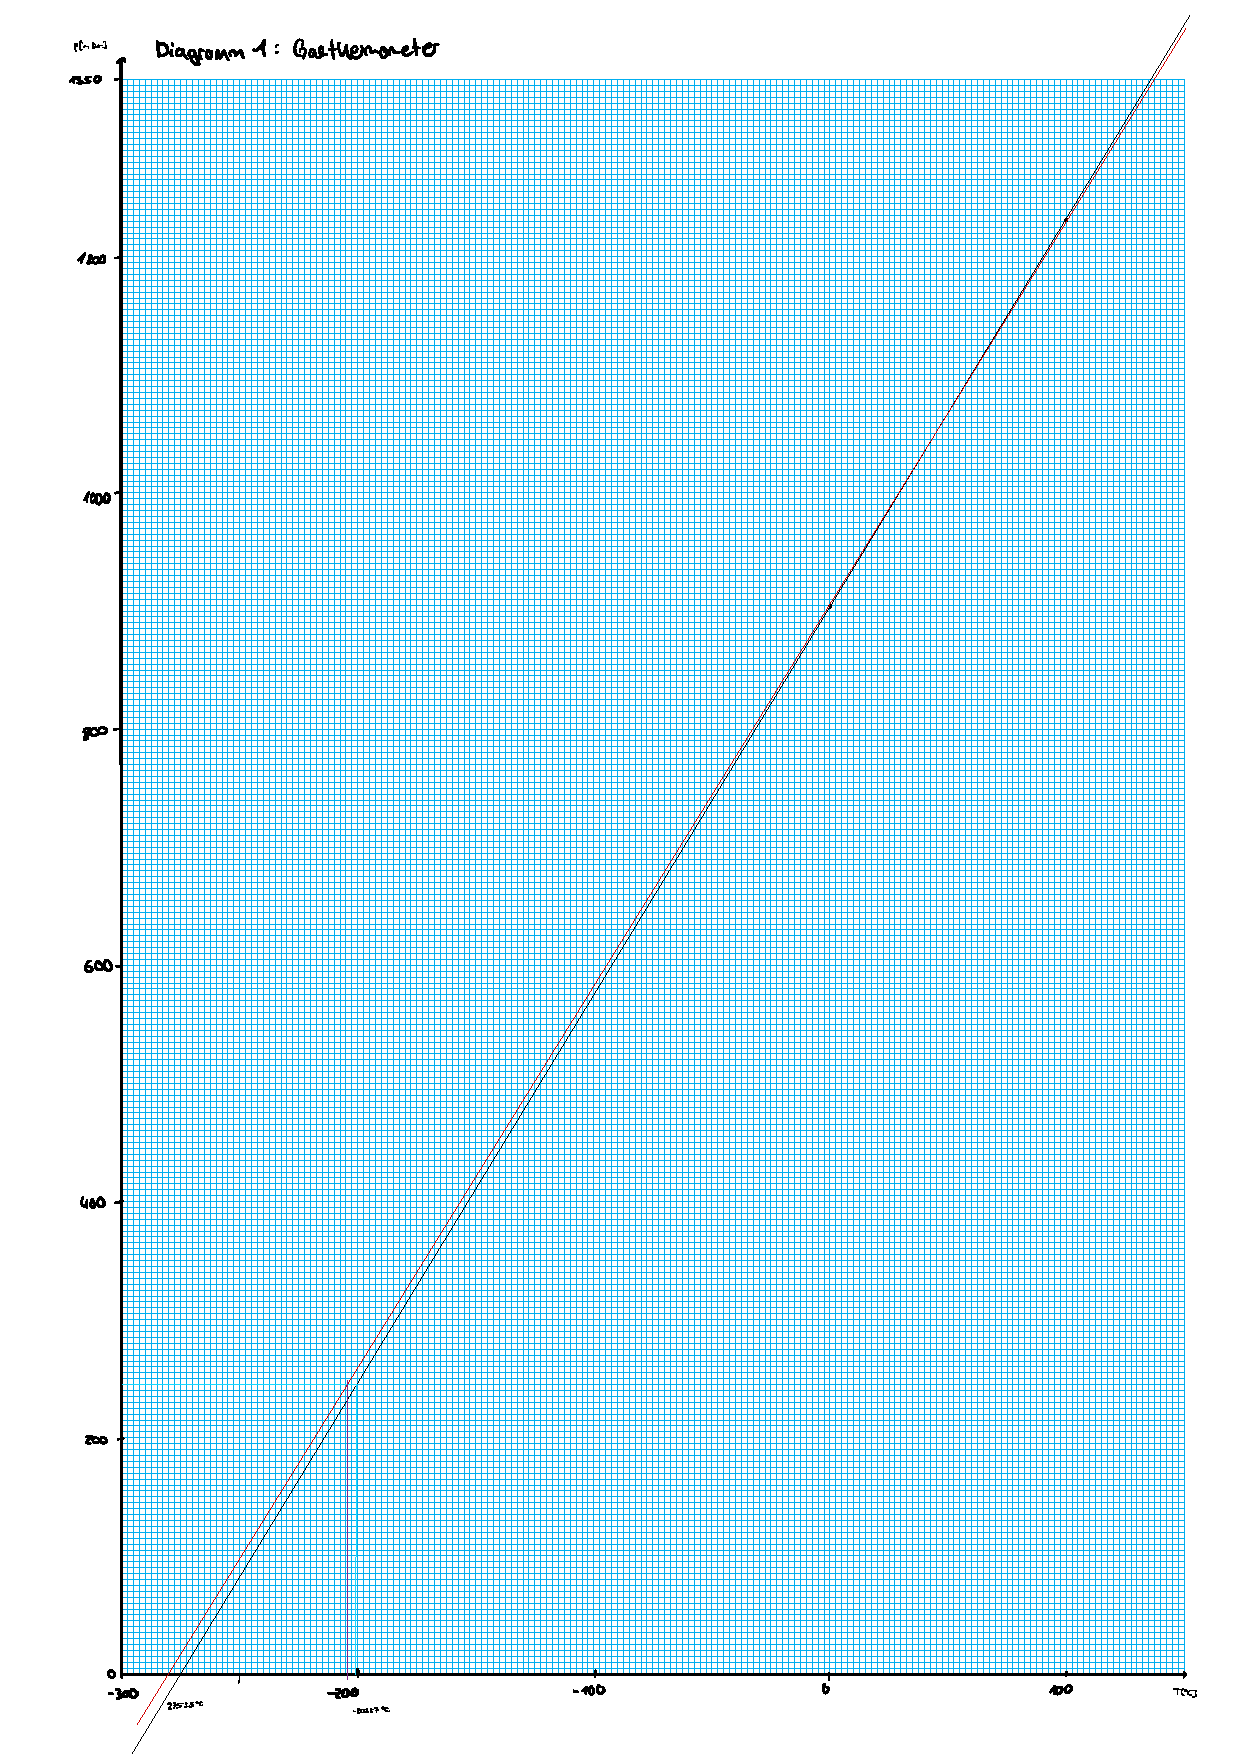
\includegraphics[page=1, width=.95\textwidth,]{41Dias.pdf}
    \caption{Diagramm 1 Gasthermometer}
\end{figure}
\newpage
\begin{figure}[h!]
    \centering
    \includegraphics[page=2, width=.95\textwidth,]{41Dias.pdf}
    \caption{Diagramm 2 Gasthermometer $N_2$}
\end{figure}
\newpage
\begin{figure}[h!]
    \centering
    \includegraphics[page=3, width=.95\textwidth,]{41Dias.pdf}
    \caption{Diagramm 3 Pt-100}
\end{figure}
\newpage
\begin{figure}[h!]
    \centering
    \includegraphics[page=4, width=0.95\textwidth,]{41Dias.pdf}
    \caption{Diagramm 4 Pyrometer}
\end{figure}
\clearpage
\newpage

Für Diagramm 1 werden die beiden Fixpunkte bei $0^\circ$C und $100^\circ$C eingetragen.
Dafür muss zuerst der Wert bei $100^\circ C$ noch auf Normalbedingungen korrigiert werden.
Dafür gilt:

\begin{equation}
    p_{NB} = p_{gem} \frac{1013,25 \text{hPa}}{p_{LD}}
\end{equation}

Wobei $p_{gem}$ der gemessene Druck und $p_{LD}$ der Außendruck ist. In dem Fall beträgt der Außendruck $1012,2$hPa.
Daraus verschiebt sich der Wert für$100^\circ C$ auf:
\[T_{100} = 1231 ^\circ C\]
Daraus ergibt sich eine Eichgerade mithilfe welcher aus dem gemessenen Druck
des siedenden Stickstoffs $245 \pm 1$mbar die Temperatur bestimmen. Für diesegilt:

\[\underline{\underline{T_{N_2} = -202 \pm 7 ^\circ C}}\]

Der Literaturwert ist gegeben durch $T_{N_2 Lit} = -195, 8 ^\circ C$. Daraus ergiebt sich
nach Gleichung \ref{eq:sigma}  eine Abweichung $1 \sigma$.\\
Es ließ sich ebenfalls der Nullpunkt bestimmen. Dieser liegt bei:

\[\underline{\underline{T_0= -275 \pm 5 ^\circ C}}\]

Im Vergleich zum Literaturwert von $-273,15^\circ C$  entspricht das einer Abweichung von $0,4 \sigma$.

\section{Diagramm 2}
Für das zweite Diagramm wurde die Temperatur von siedendem Stickstoff als weiterer Referenzpunkt hinzugefüt.
Daraufhin verändert sich die Temperatur des absoluten Nullpunkt auf:
\[ \underline{\underline{T_0 = -269 \pm 2 ^\circ C}}\]
Dieser wert entspricht einer Abweichung von $2 \sigma$.\\
Aus diesem Diagramm ließ sich ebenfalls aus dem gemessenen Druck des siedenen Kohlenstoffdioxids $680\pm 1$mbar dessen
Temperatur ablesen:
\[\underline{\underline{T_{CO_2}= - 66 \pm 1 ^\circ C}}\]

Aus den gemssenen Drücken für die Messchritte des Wassers, konnten mithilfe der Eichgerade die Zugehörigen Temperatuen abgelesen werden.
Da der Fehler auf dem Diagramm nicht ablesbar klein war, wird der Fehler hier nach oben mit $0,5 ^\circ C$ abgeschätzt.

\begin{table}[h!]
    \centering
    \caption{Gasthermometer Druck-Temperatur}
    \begin{tabular}{r r}
        \toprule
        Druck[mbar] & Temperatur[$^\circ C$]\\
        \midrule
        $904$ & $0$ \\
        $945 \pm 1$ & $14,5 \pm 0,5$ \\
        $982\pm 1$  & $25,0 \pm 0,5 $ \\
        $1018\pm 1$ & $34,0 \pm 0,5 $ \\
        $1049\pm 1$ & $45,0 \pm 0,5$ \\
        $1082\pm 1$ & $54,5 \pm 0,5 $ \\
        $1115\pm 1$ & $65,0 \pm 0,5 $  \\
        $1148\pm 1$ & $74,5 \pm 0,5 $ \\
        $1179\pm 1$ & $83,0 \pm 0,5$ \\
        $1207\pm 1$ & $92,5 \pm 0,5$ \\
        $1230$ & $100$ \\
        \bottomrule


        
    \end{tabular}
\end{table}
\clearpage
\newpage
\clearpage
\newpage

\section{Diagramm 3}
Für Diagramm 3 wurden der Widerstand des Pt-100 nach Temperatur aufgetragen.
Dafür berechnet sich der Widerstand nach dem Ohmschen Gesetz mit dem konstanten Strom von 1 mA.
Der Widerstand der Kabel ist durch das hochohmige Voltmeter vernachlässigbar.\\

Aus dem Diagramm lässt sich die Steigung ablesen, welche den Zusammenhang zwischen Temperatur un Widerstand beschreibt ablesen.
Allgemein kann die Widerstand im Idealfall durch das folgende Polynom nach Gleichung \ref{eq:Polynom} bestimmt werden.
In dem betrchteten Temperaturfenster kann dieser Zusammenhang linearisiert betrachtete werden.
Für die gemessene Steigung gilt:
\begin{equation}
    m = \frac{\Delta R}{\Delta T}
\end{equation}
\[\underline{\underline{m = 0,45 \pm 0,14 \tfrac{\Omega}{K}}}\]

Wobei der Fehler durch die Differenz zu Steigung der Fehlergeraden berechnet wurde:

\begin{equation}
    \Delta m = m- m_{Felher}
    \label{eq:SteigungFehler}
\end{equation}

Es gilt, mit $A $ von dem Polynom aus Gleichung \ref{eq:Polynom}, $m = R_0 A$ wobei $R_0 = 100 \Omega$ der Widerstand bei $T= 0^\circ C$ ist.
\[ R_0 A = 0,39083 \tfrac{\Omega}{K}\]
Daraus folgt eine Abweichung von $0,4 \sigma$.

\section{Diagramm 4}
Im 4. Diagramm wurde die gemessene Temperatur des Gasthermometers gegen die des Pyrometers aufgetragen.
Im Idealfall gibt sich für die Steigung der Geraden 1, da sie die Gleichen Temperaturen messen sollten.
Die abgelesene Steigung ist:
\begin{equation}
    m = \frac{\Delta T_{Pyro}}{\Delta T_{Druck}}
\end{equation}

\[\underline{\underline{ m = 0,94 \pm 0,14 }}\]

Daraus lässt sich die Abweichung bestimmen: $0,4 \sigma$.